\documentclass[
    10pt % font size
    16:9, % 1920x1080
]{beamer}

% \usetheme{default}
% \usetheme{Boadilla}
\usetheme{Madrid}
\usepackage{animate}
% \usetheme{Montpellier}
% \usetheme{Warsaw}
% \usetheme{Copenhagen}
% \usetheme{Goettingen}
% \usetheme{Hannover}
% \usetheme{Berkeley}

% \usecolortheme{crane}
% \beamertemplatesolidbackgroundcolor{craneorange!25}

% Define custom colors
\definecolor{customGreen}{RGB}{0,128,0}
\definecolor{customDarkGreen}{RGB}{0,100,0}

% Apply the custom colors
\usecolortheme{default}
\setbeamercolor{structure}{fg=customGreen}
\setbeamercolor{background canvas}{bg=white}
\setbeamercolor{title}{bg=customDarkGreen,fg=white}
\setbeamercolor{frametitle}{bg=customGreen,fg=white}

% Custom footline with an image on the bottom right
\addtobeamertemplate{footline}{}{%
  \hfill%
  \raisebox{5mm}[0pt][10pt]{%
    
\includegraphics[height=1cm]{kyu_univ_logo.png}%
  }\hspace*{5mm}
}

\title{StoryWeaverGPT}
\subtitle{Final Model Evaluation, Results, Limitations and Potential Fixes}
\author{Group1}

\begin{document}

\frame{\titlepage}
\section[Outline]{}
\frame{\tableofcontents}

\section{Model Results}

\frame{
  \frametitle{Review}
  \begin{columns}
    \begin{column}{0.5\textwidth}
      \begin{itemize}
        \item Trained on Shakesphere Dataset
        \item 1200 Epoch, learning rate 0.0001, no batch implemented
        \item Total Elapsed time: 28 hours
      \end{itemize}
    \end{column}
    \begin{column}{0.5\textwidth}
      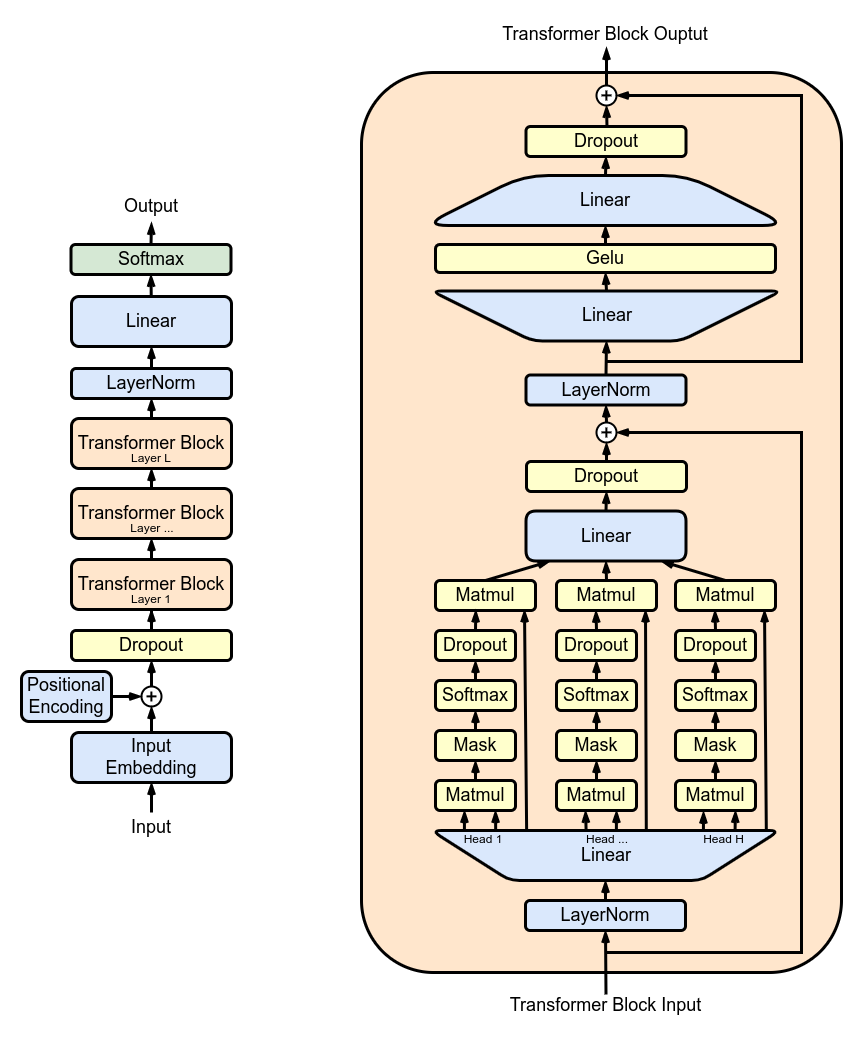
\includegraphics[width=\textwidth]{Full_GPT_architecture.png}
    \end{column}
  \end{columns}
}

\frame{
  \frametitle{Loss}
  \begin{figure}
    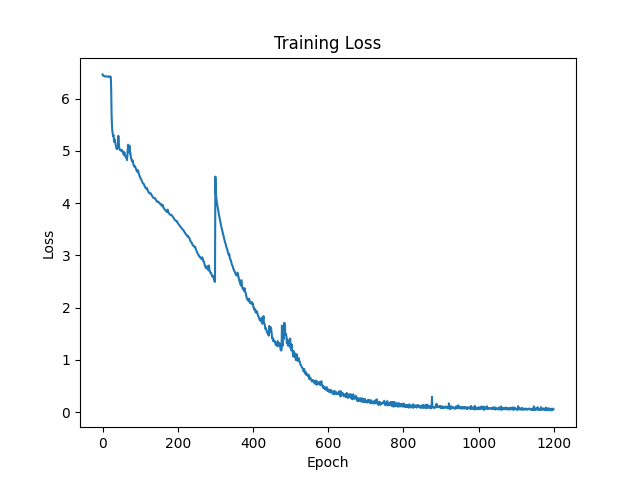
\includegraphics[width=0.8\textwidth]{loss.png}
  \end{figure}
  \vfill
}

\frame{
  \frametitle{Sample Generation}
  \begin{figure}
    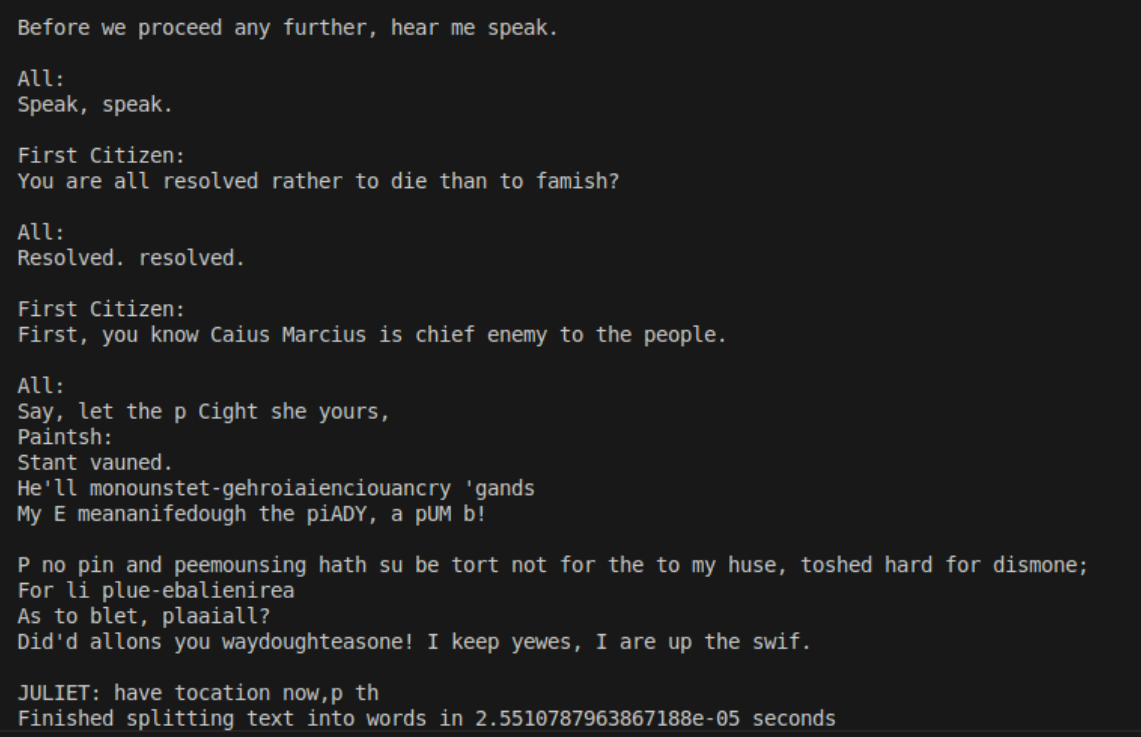
\includegraphics[width=0.8\textwidth]{sample_generation.png}
  \end{figure}
}

\frame{
  \frametitle{Model Evaluation}
  \begin{itemize}
    \item Main limitation were due to lack of diversity in dataset, and no batch implemented which lead to training inefficiency and overhead.
    \item While the model was able to generate text, it was not able to generate coherent text.
    \item Also, by performing most arithmetic and algorithms on python, it lacked efficiency.
    \item Attention mechanism implemented is not SOTA, and could be improved.
    \item Lastly, the vocab dimension was way too big given the dataset size, which paired with lack of dataset gave weak results.
  \end{itemize}
}

\frame{
  \frametitle{Potential Fixes}
  \begin{itemize}
    \item Implement batch training
    \item Use more diverse dataset
    \item Implement SOTA attention mechanism
  \end{itemize}
}

\section{Text Generation Implementation and Hyperparameters}

\frame{
  \frametitle{Hyperparameters}
  \begin{itemize}
    \item Hyperparameters: Parameters that adjusts model generation.
    \item Currently implemented: Temperature, repetition penalty, stop sequence and max tokens.
    \item Temperature: Controls randomness of the model, implemented by dividing logits by temperature.
    \item Repetition penalty: Controls how much the model avoids repeating itself, implemented by $logit = \frac{logit}{1 + repetationpenalty * frequencyvec}$.
    \item Max tokens: Controls the maximum number of tokens generated.
    \item Stop Sequence: Define a sequence of token that will stop the generation.
  \end{itemize}
}

\frame{
  \frametitle{Hyperparameters}
  \begin{figure}
    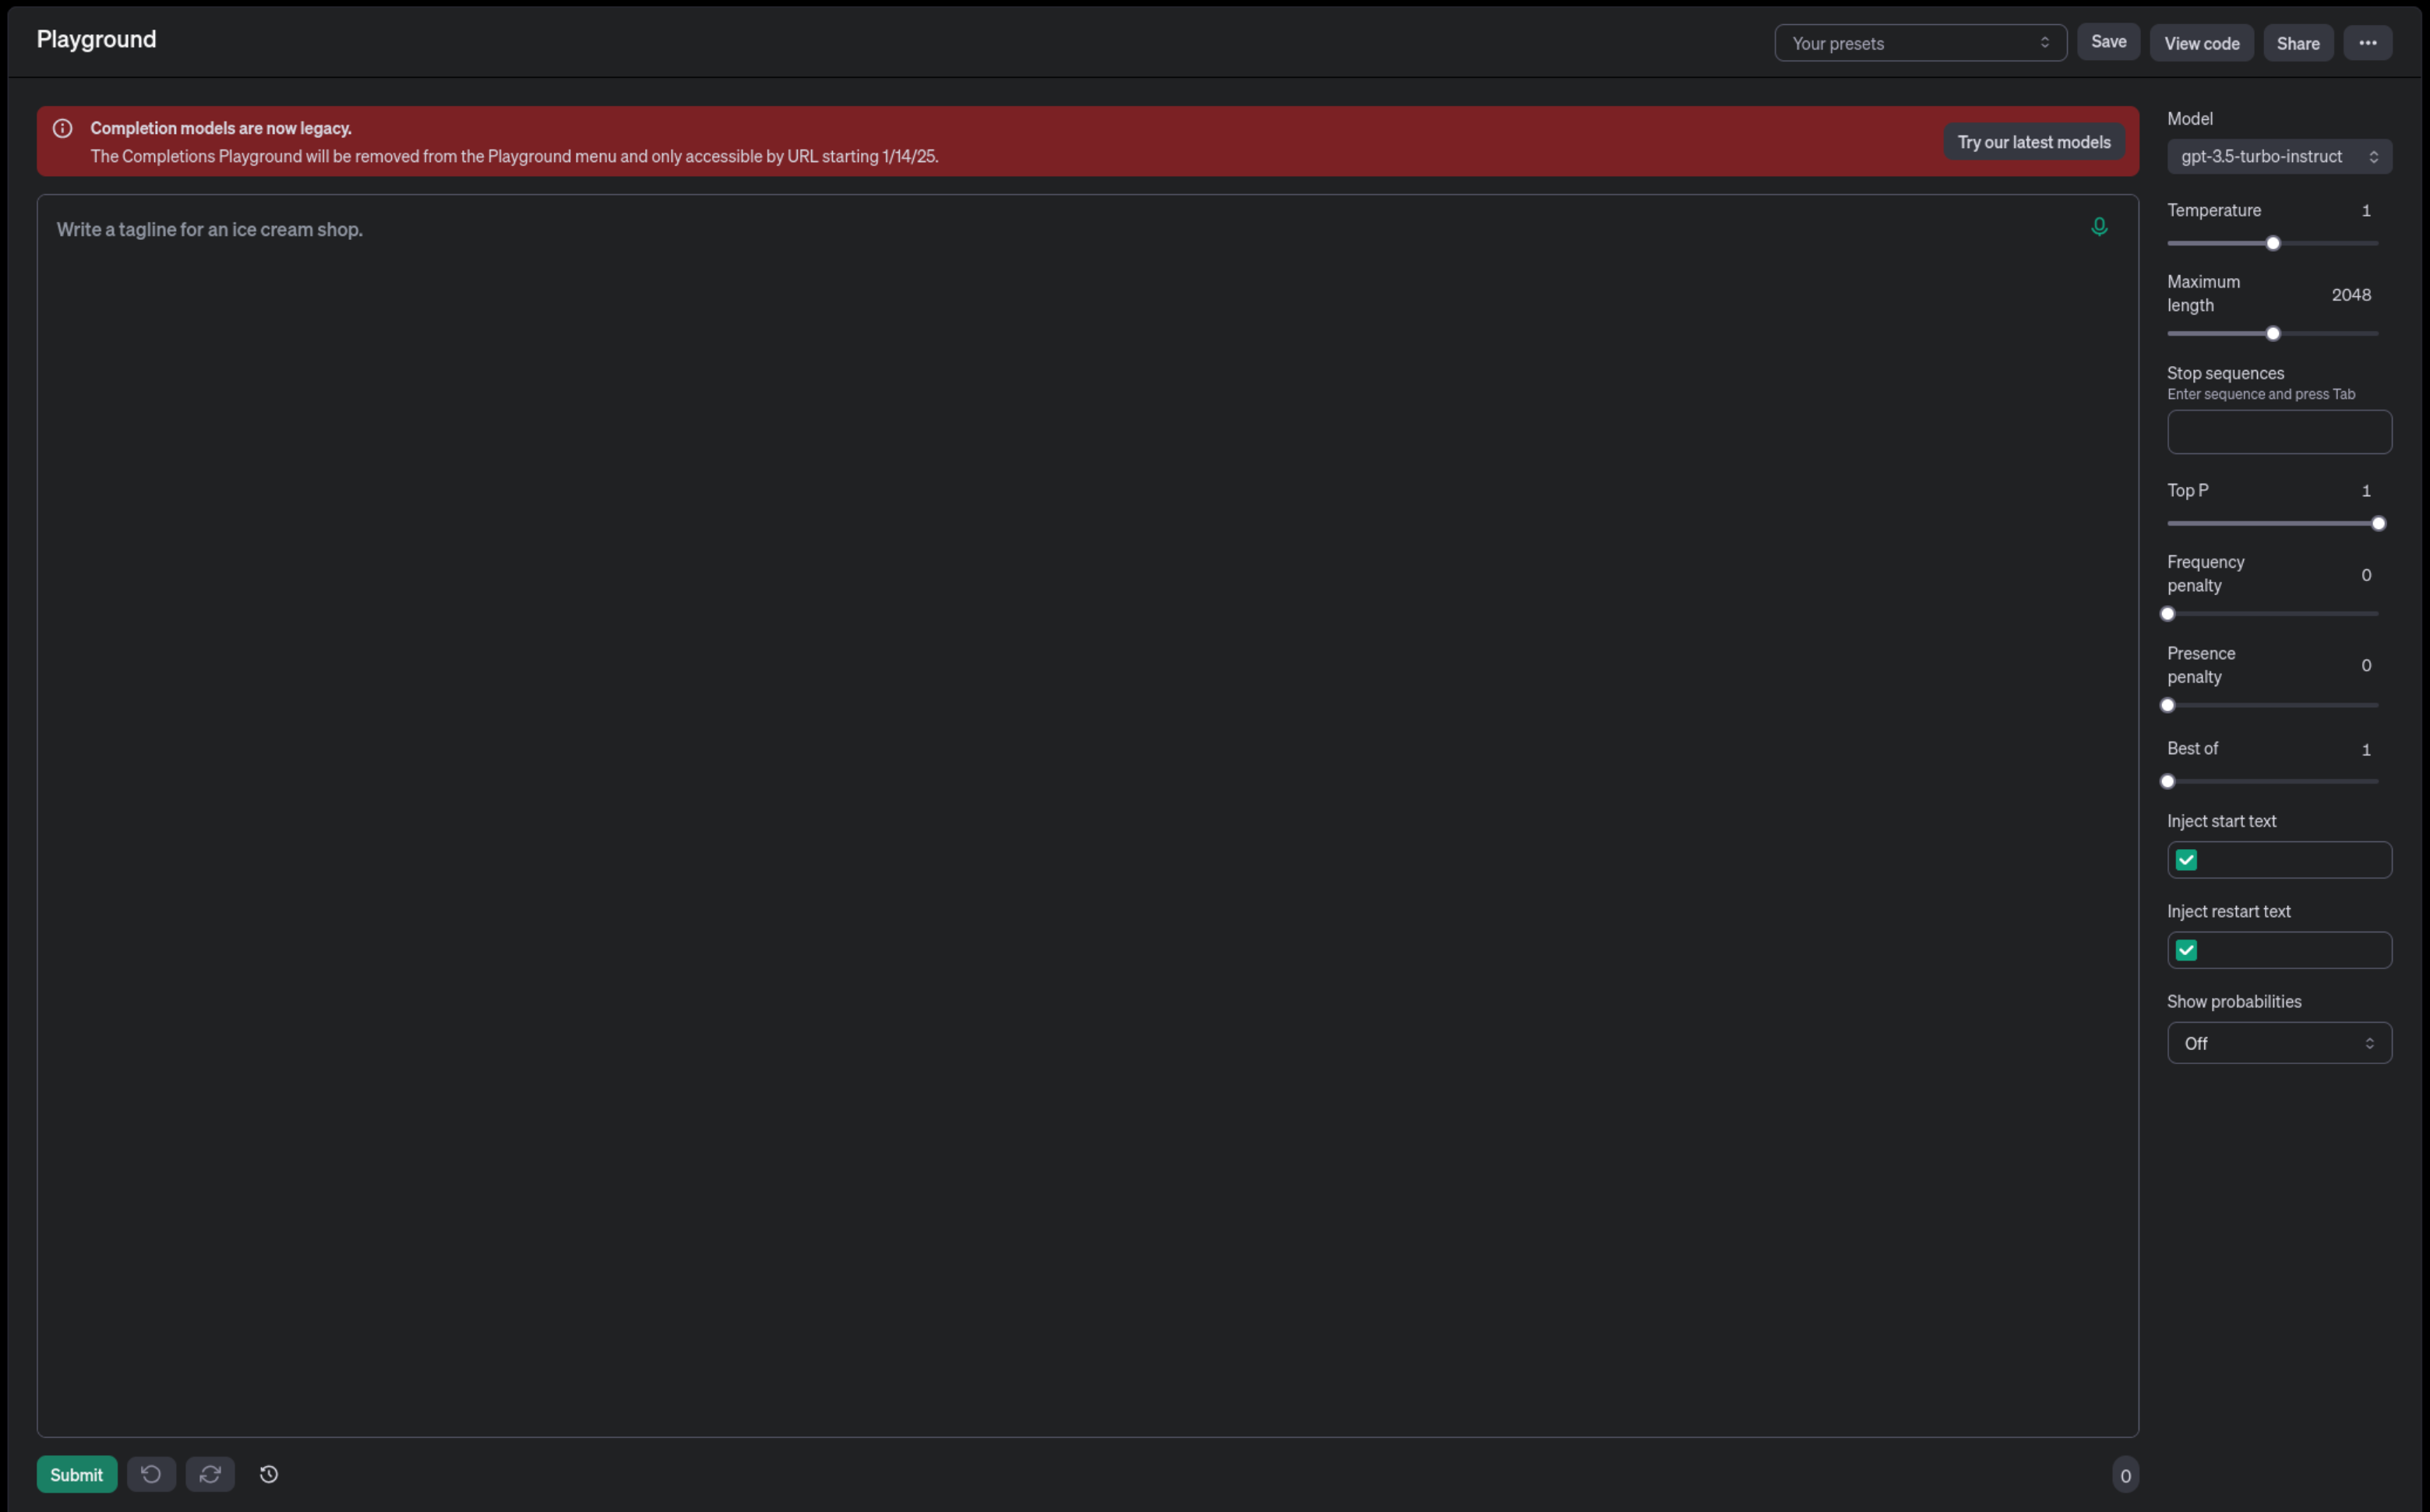
\includegraphics[width=1\textwidth]{completion.png}
  \end{figure}
}

\frame{
  \frametitle{Text Generation and Hyperparameters Implementation}
  \begin{figure}
    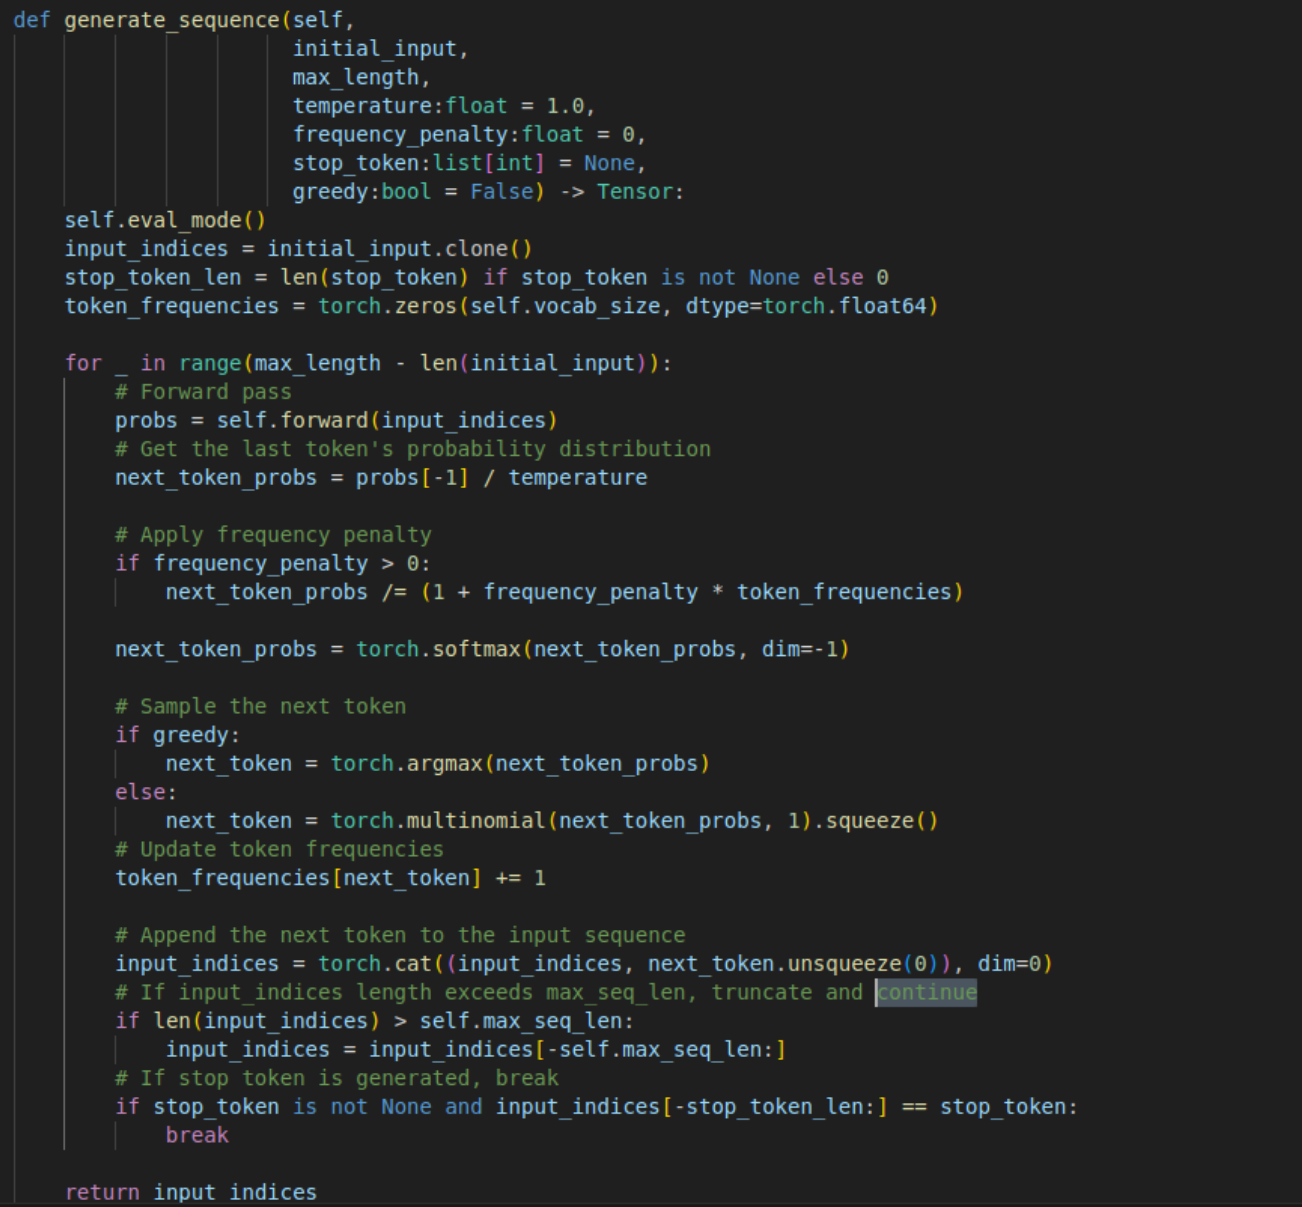
\includegraphics[width=0.7\textwidth]{generation.png}
  \end{figure}
}

\section{Fine-Tuning and other potential implementations}

\frame{
  \frametitle{Fine-Tuning}
  \begin{columns}
    \begin{column}{0.5\textwidth}
      \begin{itemize}
        \item Fine tuning is a method to teach model to generate text in a specific style.
        \item On GPT Models, it is done by training the model on a specific fine-tuning dataset.
        \item On Shakesphere, it could be implemented by two speakers conversing, one being query and the other being response.
      \end{itemize}
    \end{column}
    \begin{column}{0.5\textwidth}
      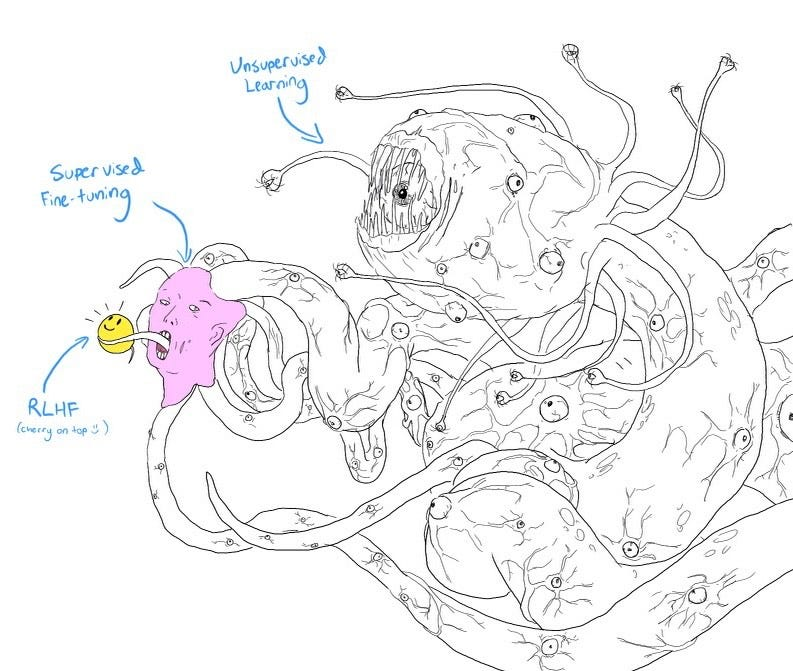
\includegraphics[width=\textwidth]{fine_tuning.jpg}
    \end{column}
  \end{columns}
}

\frame{
  \frametitle{Conclusion}
  \begin{itemize}
    \item The model was able to generate text, but not coherent text.
    \item The model could be improved by implementing batch training, using more diverse dataset, implementing SOTA attention mechanism, and reducing vocab dimension.
    \item Hyperparameters such as temperature, repetition penalty, stop sequence and max tokens were implemented.
    \item Fine-tuning could be implemented to teach the model to generate text in a specific style.
  \end{itemize}
}

\frame{
  \centering
  \Huge{Thank You!}
}
\end{document}